\documentclass[tikz,border=2pt]{standalone}
\usetikzlibrary{arrows.meta}
\usetikzlibrary{positioning}
\usepackage{amsmath}
\usepackage{amssymb}
\usepackage{tikz}
\newcommand{\R}{\mathbb R}
\newcommand{\C}{\mathbb C}
\newcommand{\Z}{\mathbb Z}
\newcommand{\Q}{\mathbb Q}
\newcommand{\F}{\mathbb F}
\DeclareMathOperator{\Fix}{Fix}
\DeclareMathOperator{\Crit}{Crit}
\DeclareMathOperator{\Morse}{Morse}
\DeclareMathOperator{\aug}{aug}
\DeclareMathOperator{\Hom}{Hom}
\DeclareMathOperator{\End}{End}
\DeclareMathOperator{\im}{im}
\DeclareMathOperator{\Spec}{Spec}
\DeclareMathOperator{\Jac}{Jac}
\begin{document}
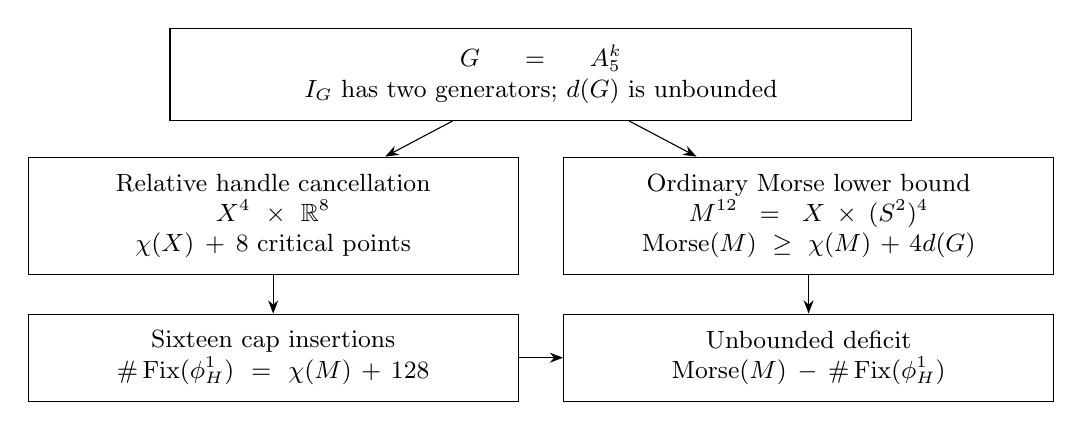
\begin{tikzpicture}[
 every node/.style={align=center,font=\small},
 box/.style={draw,inner sep=6pt,text width=58mm},
 >={Stealth}]
\node[box,text width=90mm] (group) at (0,0)
{$G=A_5^k$\\$I_G$ has two generators; $d(G)$ is unbounded};
\node[box] (morse) at (-3.4,-1.8)
 {Relative handle cancellation\\$X^4\times\R^8$\\$\chi(X)+8$ critical points};
\node[box] (bound) at (3.4,-1.8)
 {Ordinary Morse lower bound\\$M^{12}=X\times(S^2)^4$\\$\Morse(M)\ge\chi(M)+4d(G)$};
\node[box] (closed) at (-3.4,-3.6)
 {Sixteen cap insertions\\$\#\Fix(\phi_H^1)=\chi(M)+128$};
\node[box] (gap) at (3.4,-3.6)
 {Unbounded deficit\\$\Morse(M)-\#\Fix(\phi_H^1)$};
\draw[->] (group)--(morse);
\draw[->] (group)--(bound);
\draw[->] (morse)--(closed);
\draw[->] (bound)--(gap);
\draw[->] (closed)--(gap);
\end{tikzpicture}
\end{document}
